\section{Overview of the Testing Framework}
\begin{frame}{Overview of the Testing Framework}
\begin{figure}
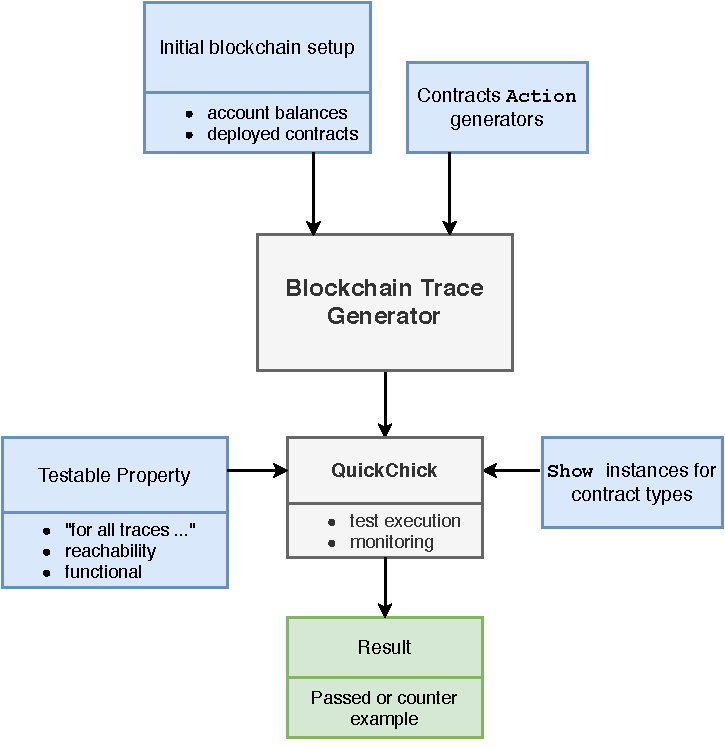
\includegraphics[scale=0.64]{media/testing-framework.pdf}
\end{figure}
\end{frame}

\begin{frame}{Overview of the Testing Framework}{Testable Properties on Execution Traces}
%\centering
\begin{tabular}{ |c|c|c| } 
\hline
Property & Testable interpretation \\
\hline
$\forall t : Trace, \ P(t)$ & \multirow{2}{16em}{Test $P$ holds on many generated traces} \\
&\\ %empty row
\hline
\multirow{2}{10em}{$\exists c : Chain, $ \\ $reachable(c) \land P(c)$} & \multirow{4}{16em}{Assert that the test of $\neg P(c)$ fails in some step of a generated trace. Print counterexample as witness of $P(c)$} \\
&\\&\\&\\ %three empty rows
\hline
\multirow{4}{10em}{Given a contract $C$, \\$\forall m : Msg,$ \\ $ \{P(C,m)\} $\\$C.\coqcode{receive}(m)$\\$\{Q(C,m)\}$} & \multirow{4}{16em}{For each generated trace, check for each step if there are messages to $C$ satisfying $P$. If so, execute $C.$\coqcode{receive} and check if $Q$ holds.}  \\
&\\&\\&\\
&\\&\\&\\
\hline
\end{tabular}
\end{frame}

\section{ERC20 Example, revisited}

\defverbatim[colored]\gtokenact{
\begin{coq}
backtrack [
  (1, gTransfer      token_state) ;;
  (1, gTransfer_from token_state) ;;
  (1, gApprove       token_state) ;;
]
\end{coq}
}
\defverbatim[colored]\gtransferfrom{
\begin{coq}
Definition gTransfer_from (state : EIP20Token.State) 
                          : G (option (Address * Msg)) :=
  (allower, allowance_map) <- sampleFMapOpt state.(allowances) ;;
  (delegate, allowance)    <- sampleFMapOpt allowance_map ;;
  (receiver, _)            <- sampleFMapOpt state.(balances) ;;
  let allower_balance := with_default 0 
                         (FMap.find allower state.(balances)) in
  amount <- if allower_balance =? 0 
            then returnGen 0 
            else choose (0, min allowance allower_balance) ;; 
  returnGen (Some 
    (delegate, transfer_from allower receiver  amount)).
\end{coq}
}

\begin{frame}{ERC20 Token Example Revisited}{Implementing the generator}
Composing optional generators with \coqcode{backtrack}:
\gtokenact
\end{frame}

\begin{frame}{ERC20 Token Example Revisited}{Implementing the generator}
\gtransferfrom
\end{frame}


\defverbatim[colored]\testtransfer{
\begin{coq}
QuickChick (
  {{msg_is_transfer}}
  EIP20Token.contract
  {{post_transfer_correct}}
).
\end{coq}
}

\defverbatim[colored]\testtransferfromsafe{
\begin{coq}
QuickChick (
  initial_chain $\rightsquigarrow$ transfer_from_is_safe_P
).
\end{coq}
}


\begin{frame}{ERC20 Token Example Revisited}{Testing the Contract}
Testing a Functional property:
\testtransfer
Testing a Reachability/Temporal property:
\testtransferfromsafe
\end{frame}


\section{Conclusions \& Future Work}
\begin{frame}{Conclusions}
\begin{itemize}
    \item Our approach is based on generating arbitrary blockchain execution traces
    \item this allows stating both functional and temporal properties
    \item and test interacting contracts (not shown in this presentation)
    \item we have sacrificed some automation to obtain the necessary performance...
    \item we have (re-)discovered many known vulnerabilities/bugs using our testing framework
    \item hence, the approach is capable, and seems effective at findings bugs
    \item Since the development is in Coq, we can combine testing and verification efforts (not shown in this presentation)
\end{itemize}
\end{frame}

\begin{frame}{Future Work}
\begin{itemize}
    \item improve automation of deriving generators, e.g. using Luck\cite{lampropoulos2016beginners}
    \item certified generators
    \item shrinking for minimal counter examples
    \item align testable execution traces with ConCert's notion of execution traces
    \item integrate this work into the official ConCert repository (pull request currently under review...)
\end{itemize}
\end{frame}